%-------------------------
% Rover Resume - Fancy Template
% Link: https://github.com/subidit/rover-resume
%------------------------

\documentclass[11pt]{article}

\usepackage[T1]{fontenc}
\usepackage{inter} % https://tug.org/FontCatalogue/
\renewcommand*\familydefault{\sfdefault}
\usepackage{graphicx}

\usepackage{geometry}
\geometry{
a4paper,
top=1.8cm,
bottom=1in,
left=2.5cm,
right=2.5cm
}

\setcounter{secnumdepth}{0} % remove section numbering
%\pdfgentounicode=1 % make ATS friendly

\usepackage{enumitem}
\setlist[itemize]{
    noitemsep,
    left=0pt..1.5em
}
\setlist[description]{itemsep=0pt}
\setlist[enumerate]{align=left}

\usepackage[dvipsnames]{xcolor}
% \usepackage[dvipsnames, svgnames, x11names]{xcolor} 
% \usepackage[dvipsnames]{xcolor} % xcolor.pdf Sec.4 Colors by Name
\colorlet{icnclr}{gray}
% \colorlet [⟨type⟩]{⟨name⟩}[⟨num model⟩]{⟨color ⟩}
% \definecolor[⟨type⟩]{⟨name⟩}{⟨model-list⟩}{⟨spec-list⟩}


\usepackage{titlesec}
% \titlespacing{command}{left spacing}{before spacing}{after spacing}[right]
% \titlespacing{\section}{0pt}{*3}{*1}
\titlespacing{\subsection}{0pt}{*0}{*0}
\titlespacing{\subsubsection}{0pt}{*0}{*0}
% \titleformat{<command>}[<shape>]{<format>}{<label>}{<sec>}{<before-code>}[<after-code>]  
\titleformat{\section}{\color{Sepia}\large\fontseries{black}\selectfont\uppercase}{}{}{\ruleafter}[\global\RemVStrue]
\titleformat{\subsection}{\large\fontseries{semibold}\selectfont}{}{}{\rvs}
\titleformat{\subsubsection}{\large\fontseries{medium}\selectfont}{}{}{}

\usepackage{xhfill} 
\newcommand\ruleafter[1]{#1~\xrfill[.5ex]{1pt}[gray]} % add rule after title in .5 x-height 

\newif\ifRemVS % remove vspace between \section & \subsection
\newcommand{\rvs}{
    \ifRemVS
        \vspace{-1.5ex}
    \fi
    \global\RemVSfalse
}


\usepackage{fontawesome5}

\usepackage[bookmarks=false]{hyperref} % [imp!]
\hypersetup{ % https://en.wikibooks.org/wiki/LaTeX/Hyperlinks
    colorlinks=true,
    urlcolor=Sepia,
    pdftitle={My Resume}}

\usepackage[page]{totalcount}
\usepackage{fancyhdr}
\pagestyle{fancy}
\renewcommand{\headrulewidth}{0pt}	
\fancyhf{}							
\cfoot{\color{darkgray} Alessio Rovere CV (ITA) -- Page \thepage{} of \totalpages}


\usepackage[backend=biber,style=apa,sorting=ydnt,uniquename=false,isbn=false,maxbibnames=99,url=false,giveninits=true,eprint=false]{biblatex}
\AtEveryBibitem{\clearfield{note}}
\addbibresource{sample.bib}


\begin{document}
% ---------- ITALIAN ----------------------
\begin{center}
    {\fontsize{36}{36}\selectfont\interthin Alessio \interheavy Rovere} \\ \bigskip
    {\fontsize{14}{14}\selectfont\interthin Curriculum Vitae - Versione Italiana}\\ \bigskip
    {\color{icnclr}\faEnvelope[regular]} \href{mailto:alessio.rovere@unive.it}{alessio.rovere@unive.it}
\end{center}

\section{Titoli di studio accademici}
{\normalfont Il mio percorso accademico si è svolto presso l'Università di Genova, Italia, rinomata per la sua eccellenza nelle scienze ambientali marine e nelle geoscienze. Ho vinto due premi di laurea, uno per la tesi triennale e uno per la magistrale. Durante il mio dottorato, ho partecipato a diversi soggiorni di ricerca all'estero e ho ottenuto la \textit{"European Ph.D. Label"}.} \\

\bigskip
\subsection{Università degli Studi di Genova $|$ {\normalfont\textit{Ph.D. in Marine Sciences}} \hfill 06/2011}
{\footnotesize Il mio dottorato di ricerca ha ottenuto il riconoscimento \textit{"European Ph.D. label"}. In quanto tale, ha richiesto almeno sei mesi di ricerca all'estero, la valutazione della tesi da parte di due professori provenienti da paesi europei distinti, la partecipazione di almeno un membro della commissione proveniente da un paese europeo diverso dall'Italia, e la difesa della tesi in una lingua ufficiale dell'UE diversa dall'italiano. Il mio principale supervisore è stato il Prof. Marco Firpo. \\
\textbf{Tesi}: \textit{Rocky Coasts in the Ligurian Sea: Morphology, Evolution, and Management Aspects}.\\ 
\textbf{Periodi all'estero durante il dottorato}: University of Western Australia, AU (2010, 1 mese); Brunel University, UK (2010, 4 mesi); University of the Aegean, GR (2010, 17 giorni); University of the Aegean, GR (2009, 1 mese).}
\bigskip

\subsection{Università degli Studi di Genova $|$ {\normalfont\textit{LM in Sc. Ambientali Marine}} \hfill 07/2006}
{\footnotesize Ho completato un corso di laurea magistrale di due anni in Scienze Ambientali Marine, durante il quale ho ricevuto una borsa di studio ERASMUS. Ho conseguito un voto finale di 110/110. I miei principali supervisori sono stati il Prof. Marco Firpo e il Prof. Carlo Nike Bianchi. \\
\textbf{Tesi}: \textit{Cartografia e Geomorfologia del Fondale Marino nell'Area Marina Protetta di Bergeggi (SV).}\\
\textbf{Borsa di studio ERASMUS}: \textbf{2004} Universidad de Las Palmas de Gran Canaria, ES (3 mesi, 18 giorni).\\
\textbf{Premio di Laurea}: "Premio Parchi Cum Laude", Regione Liguria (2010), secondo premio ex-aequo.}
\bigskip

\subsection{Università degli Studi di Genova $|$ {\normalfont\textit{LT in Scienze Ambientali}} \hfill 02/2004}
{\footnotesize Ho completato un corso di laurea triennale in Scienze Ambientali, diplomandomi con il massimo dei voti, 110/110. Ho svolto la mia tesi sotto la guida del Prof. Carlo Nike Bianchi. \\
\textbf{Tesi}: \textit{Lineamenti geologici e geomorfologici dei fondali dell’Isola di Bergeggi legati all’istituzione dell’Area Marina Protetta}.\\
\textbf{Premio di Laurea}: "Prix Alain Vatrican 2003 (RAMOGE, Monaco)" primo premio ex-aequo.}

\newpage
\section{Esperienza di insegnamento e ricerca}
{\normalfont Dopo aver completato il dottorato, la mia carriera accademica si è principalmente sviluppata all'estero. Ho trascorso due anni negli Stati Uniti presso la Columbia University, classificata al 17° posto nel World University Rankings 2024 di THE, e otto anni alla Universität Bremen, riconosciuta come \textit{"Università di Eccellenza"} tedesca. Sono tornato in Italia nel 2021. Dal marzo 2014, a soli due anni e nove mesi dopo il dottorato, ho guidato in modo indipendente il mio gruppo di ricerca.}\\

\bigskip
\subsection{Università Ca' Foscari Venezia $|$ {\normalfont\textit{Professore Ordinario}} \hfill 11/2021 - Presente}
{\footnotesize Nel ruolo di Professore Ordinario, le mie responsabilità includono insegnamento, ricerca e amministrazione accademica.}

\bigskip
\subsection{Università Ca' Foscari Venezia $|$ {\normalfont\textit{Professore Associato}} \hfill 11/2021 - 11/2024}
{\footnotesize La mia nomina a Professore Associato a Ca' Foscari è avvenuta tramite un incarico diretto in seguito alla valutazione positiva del Ministero dell'Università e della Ricerca (prot. n. 11888 del 4.09.2021), ai sensi dell'articolo 1, comma 9 della Legge n. 230/2005.}

\bigskip

\subsection{Universität Bremen $|$ {\normalfont\textit{Professore}} \hfill 04/2020 - 10/2021}
{\footnotesize Oltre alla mia posizione di \textit{"Independent Researcher"}, mi è stato conferito il titolo di \textit{"Professor"} in conformità con l'articolo 17 della Legge sull'Istruzione Superiore dello Stato di Brema.}
\bigskip

\subsection{Universität Bremen $|$ {\normalfont\textit{Research group leader}} \hfill 03/2019 - 10/2021}
{\footnotesize Come \textit{"research group leader"} di ruolo presso il MARUM (Center for Marine Environmental Sciences) dell'Università di Brema, ho guidato il gruppo di ricerca \textit{"Sea Level and Coastal Changes"}. Le mie responsabilità includevano la direzione di programmi di ricerca e l'adempimento degli obblighi di insegnamento presso l'Università, con un focus primario sulla ricerca.}
\bigskip

\subsection{Universität Bremen e Leibniz ZMT $|$ {\normalfont\textit{Young group leader}} \hfill 03/2014 - 02/2019}
{\footnotesize Come \textit{"Young Research Group Leader"} (posizione tenure-track) presso il MARUM (Center for Marine Environmental Sciences) e il Leibniz Center for Tropical Marine Research (ZMT), ho fondato e diretto il gruppo di ricerca \textit{"Sea Level and Coastal Changes"}. Il mio ruolo comprendeva la guida di progetti di ricerca, la gestione di fondi e la richiesta di finanziamenti. Ho inoltre partecipato alle attività didattiche dell'Università di Brema.}
\bigskip

\subsection{Columbia University $|$ {\normalfont\textit{Ricercatore Post-Dottorato}} \hfill 02/2012 - 02/2014}
{\footnotesize Come \textit{"postdoctoral researcher"} presso il Lamont-Doherty Earth Observatory della Columbia University, ho svolto ricerche nell'ambito del progetto finanziato dalla US National Science Foundation \textit{"PLIOcene MAXimum sea level (PLIOMAX)"}, sotto la guida della Prof.ssa Maureen E. Raymo.}

\section{Trasferimento Tecnologico}
{\normalfont Durante il mio dottorato all'Università di Genova, ho co-fondato SeaMap srl, una società di consulenza ambientale, in collaborazione con sei partner. L'azienda ha ottenuto finanziamenti iniziali attraverso un consorzio avviato dall'Università di Genova (UNITI) ed è stata successivamente riconosciuta come spinoff dell'università. Come Amministratore Unico ho gestito le operazioni fino alla sua chiusura. Nel 2011, SeaMap ha ricevuto il premio \textit{"Italia degli Innovatori"} dall'\textit{"Agenzia per la diffusione delle tecnologie per l’innovazione - Presidenza del Consiglio dei Ministri"}}\\
\bigskip

\subsection{SeaMap srl $|$ {\normalfont\textit{Amministratore Unico}} \hfill 10/2010 - 12/2016}
{\footnotesize Nella funzione di Amministratore Unico, ho guidato gli aspetti tecnici e amministrativi dei progetti commerciali, gestendo in parallelo le attività di ricerca e sviluppo. Sono stato responsabile dell'impiego dei fondi di avviamento e ho gestito, in totale, circa 150.000 (esclusa l'IVA) euro in progetti di vario tipo.}
\bigskip

\section{Altre Posizioni di Ricerca o Insegnamento}
{\normalfont Oltre alle mie posizioni di lavoro accademiche principali, ho ricoperto diversi incarichi come 'faculty adjunct'.}\\
\bigskip

\subsection{Universität Bremen $|$ {\normalfont\textit{Professore Onorario}} \hfill 03/2024 - Presente}
{\footnotesize l'Universitá di Brema mi ha conferito il titolo di \textit{"Professore Onorario"}. Questo incarico implica una partecipazione attiva nelle attività di insegnamento e ricerca.}
\bigskip

\subsection{MARUM - Universität Bremen $|$ {\normalfont\textit{Membro Esterno}} \hfill 10/2021 - Presente}
{\footnotesize Come membro esterno del MARUM, mi si richiede di partecipare attivamente nelle attività di ricerca all'interno del cluster designato, dedicando tempo a riunioni di progetto. e partecipando a comitati di tesi.}
\bigskip

\subsection{LDEO - Columbia University $|$ {\normalfont\textit{Adjunct Research Scientist}} \hfill 04/2014 - 08/2021}
{\footnotesize Come \textit{Adjunct Research Scientist} presso il Lamont-Doherty Earth Observatory della Columbia University, il mio ruolo prevedeva la partecipazione alle attività di ricerca, mantenendo al contempo la mia affiliazione primaria con un'altra istituzione.}

\section{Incarichi Universitari}
%===============
{\normalfont Come Professore Associato all'Università Ca' Foscari, ho diversi incarichi relativi alla supervisione e gestione delle attività didattiche e di ricerca.}\\
%============
\bigskip
\subsection{Università Ca' Foscari Venezia $|$ {\normalfont\textit{Coordinatore Collegio}} \hfill 04/2024 - Presente}
{\footnotesize Come Coordinatore del collegio didattico in Scienze Ambientali, nominato dal Consiglio del Dipartimento DAIS di Ca' Foscari il 26.03.2024, gestisco la supervisione e l'implementazione del Programma di Studio in Scienze Ambientali, inclusa la sua continua revisione. Promuovo il processo di Garanzia della Qualità, allineandolo agli obiettivi strategici dell'Università e del Dipartimento.}
\bigskip

\subsection{Università Ca' Foscari Venezia $|$ {\normalfont\textit{Collegio di Dottorato}} \hfill 05/2023 - Presente}
{\footnotesize Sono membro del Collegio di Dottorato per il \textit{"Dottorato di Interesse Nazionale in Scienze Polari"} presso l'Università Ca' Foscari di Venezia.}
\bigskip

\subsection{Università Ca' Foscari Venezia $|$ {\normalfont\textit{Collegio di Dottorato}} \hfill 05/2022 - Presente}
{\footnotesize Sono membro del Collegio di Dottorato in \textit{"Scienze Polari"} presso l'Università Ca' Foscari di Venezia.}
\bigskip

\subsection{Università Ca' Foscari Venezia $|$ {\normalfont\textit{Commissione ERASMUS}} \hfill 12/2022 - Presente}
{\footnotesize Sono membro della \textit{"Commissione Erasmus per le Scienze Ambientali"} (nominato dal Consiglio del Dipartimento DAIS di Ca' Foscari il 13.12.2022). Supervisiono le richieste di borse di studio ERASMUS e contribuisco all'internazionalizzazione del nostro corpo studentesco.}
\bigskip

\subsection{Università Ca' Foscari Venezia $|$ {\normalfont\textit{ERC Board}} \hfill 09/2022 - Presente}
{\footnotesize Sono membro dell'ERC Board di Ca' Foscari (nominato con Decreto Rettorale di Ca' Foscari 815/2022), valuto le domande e fungo da collegamento tra il mio Dipartimento e i Principal Investigators dei progetti ERC che inizialmente avevano scelto un'altra istituzione italiana o straniera come Istituzione Ospitante ma intendono trasferirsi a Ca' Foscari. Cerco attivamente ricercatori di talento e avvio contatti con loro.}
\bigskip

\subsection{Università Ca' Foscari Venezia $|$ {\normalfont\textit{ESA Lab}} \hfill 2022 - Presente}
{\footnotesize Sono membro del Comitato Direttivo di \textit{"ESA Lab@Ca' Foscari"} (Ca' Foscari e Agenzia Spaziale Europea), che promuove, coordina e supporta le attività di ricerca, le collaborazioni scientifiche, le iniziative didattiche e gli eventi scientifici relativi ai dati e alla ricerca spaziale.}

\newpage
\section{Altri incarichi}
%===============
{\normalfont Sono un membro attivo della comunità scientifica internazionale attiva sui cambiamenti del livello del mare e processi costieri.}\\
%============
\bigskip
\subsection{INQUA $|$ {\normalfont\textit{Presidente Commissione INQUA CMP}} \hfill 2023 - Presente}
{\footnotesize Come Presidente della Commissione \textit{"Coastal and Marine Processes"} della International Union for Quaternary Science (INQUA), guido le decisioni strategiche e supervisiono le domande di finanziamento per conferenze e workshop.}
\bigskip

\subsection{SCAR-INSTANT $|$ {\normalfont\textit{Comitato Direttivo}} \hfill 2022 - Presente}
{\footnotesize Come membro del Comitato Direttivo del progetto \textit{"Instabilities and Thresholds in Antarctica"} (INSTANT) nell'ambito dello \textit{"Scientific Committee on Antarctic Research"} (SCAR), contribuisco a indirizzare la ricerca scientifica dell'organizzazione.}
\bigskip

\subsection{PALSEA $|$ {\normalfont\textit{Co-Leader}} \hfill 2018 - 2023}
{\footnotesize Ho ricoperto il ruolo di co-leader (con altri tre scienziati) del progetto PALSEA (PALeo constraints on SEA level rise), finanziato dalla International Union of Quaternary Sciences (INQUA) e da Past Global Changes (PAGES). Ho diretto le decisioni strategiche sul focus scientifico del progetto, promosso attività per espanderne l'ambito e gestito le domande di finanziamento per le travel grants di giovani ricercatori.}
\bigskip

\subsection{MPA "Cinque Terre" $|$ {\normalfont\textit{Membro del Comitato Scientifico}} \hfill 06/2021 - Presente}
{\footnotesize Come membro del Comitato Scientifico dell'Area Marina Protetta (AMP) \textit{"Cinque Terre"}, contribuisco alla supervisione delle attività scientifiche all'interno dell' AMP e fornisco orientamenti su questioni tecniche e scientifiche relative alla sua gestione.}
\bigskip

\subsection{MEDFLOOD/MOPP $|$ {\normalfont\textit{Co-Leader}} \hfill 2012 - 2018}
{\footnotesize Ho ricoperto il ruolo di co-leader (con altri tre scienziati) dei progetti MEDFLOOD e MOPP, finanziati dalla International Union for Quaternary Science (INQUA) per sostenere workshop annuali e scuole di formazione sullo studio del livello del mare passato nel Mediterraneo. Ho diretto le decisioni strategiche sul focus scientifico del progetto, promosso attività per espanderne l'ambito e gestito le domande di finanziamento per le travel grants di giovani ricercatori.}

\section{Organizzazione di conferenze e workshops}
%===============
{\normalfont Nel corso della mia carriera, ho attivamente organizzato workshops e proposto sessioni per conferenze internazionali. Di seguito è riportato un elenco di conferenze e workshop in cui ho fatto parte del comitato organizzatore, o ho assunto il ruolo di organizzatore di sessioni, moderatore o chair.}\\

{\normalfont 
\subsection{Membro del comitato scientifico o organizzatore}}
{\footnotesize
\begin{description}
  \item [2022] PALSEA annual meeting, Singapore.
  \item [2021] Webinar series by PALSEA, WCRP (sea level), IAG, and SERCE.
  \item [2020] "PALSEA Express" online workshop.
  \item [2019] CoChE Summer school. Coastal Changes and Evolution. Oristano (IT).
  \item [2019] PALSEA workshop "Using ecological and chronological data to improve proxy-based paleo sea level reconstructions", Dublin (IE).
  \item [2017] PALSEA-QUIGS meeting on “Climate, ice sheets and sea level during past interglacial periods”. Galloway, New Jersey (USA)
\item [2016] Annual MEDFLOOD workshop, Bremen (DE)
\item [2014] Annual MEDFLOOD workshop, Haifa (IL).
\item [2012] Annual MEDFLOOD workshop, Rome (IT).
\item [2013] Organizer of the bi-weekly seminar at Lamont Doherty Earth Observatory, Biology and Paleo Environment Division
  \item \end{description}}

{\normalfont 
\subsection{Organizzatore di sessione, convener o session chair}}
{\footnotesize
\begin{description}
  \item [2023] Rome INQUA conference. Session 89: "Cenozoic sea-level indicators and ice sheet constraints to global sea-level change".
  \item [2022] PAGES Open Science Meeting. Session: "Last Interglacial".
  \item [2019] American Geophysical Union 2019. Session PP23A: "Centennial Session: One Hundred Years of Ice Sheet and Sea Level Science".
  \item [2017] GeoBremen conference. Session: "Coastal depositional environments \& processes"
  \item [2015] American Geophysical Union 2015. Session PP11E: "Sea Levels and Ice Sheets during Past Warm Periods: Looking to the Past to Understand the Future".
  \item \end{description}}

\section{Altri Ruoli Scientifici di rilievo}
\subsection{IPCC AR6 $|$ {\normalfont\textit{Contributing author}} \hfill 2022}
{\footnotesize Sono stato \textit{"contributing author"} per il Sesto Rapporto di Valutazione (AR6) dell'Intergovernmental Panel on Climate Change (IPCC), contribuendo ai Capitoli 2 e 9 del Gruppo di lavoro 1. Come contributing author, ho fornito informazioni tecniche, inclusi testi, grafici e dati, per l'integrazione nelle sezioni della bozza.}

\section{Seminari e Conferenze ad Invito}
{\normalfont Oltre alle mie responsabilità didattiche, sono frequentemente invitato a presentare la mia ricerca in seminari universitari e conferenze internazionali. Di seguito, un elenco delle presentazioni più significative che ho tenuto negli anni.}

{\footnotesize 
\begin{description}
  \item [2023] University of Genoa (IT).
  \item [2023] QUIGS workshop (Online).
  \item [2022] ECORD Summer School 2022 (DE).
  \item [2021] Ca’ Foscari University of Venice (IT).
  \item [2019] PAGES ECN grant-writing workshop, Prague (CZ).
  \item [2018] Ca’ Foscari University of Venice (IT).
  \item [2018] Durham University (UK).
  \item [2018] CEREGE, Université Aix-Marseille (FR).
  \item [2017] Bonn University (DE).
  \item [2017] University of Cambridge (UK).
  \item [2017] Université de Bretagne Occidentale, Brest (FR).
  \item [2017] University of Genoa (IT).
  \item [2016] American Geophysical Union, San Francisco (USA).
  \item [2015] LDEO, Columbia University (USA).
  \item [2013] University of Bremen (DE).
  \item [2012] Rice University, Houston (USA).
  \item [2008] Université du Sud Toulon-Var (FR).
\end{description}
}
\newpage

\section{Ruoli editoriali}
{\normalfont Nel corso della mia carriera, ho ricoperto vari ruoli come editore di riviste scientifiche.}\\

\bigskip

\subsection{Earth System Science Data $|$ {\normalfont\textit{Editor}} \hfill 2022 - Presente}
{\footnotesize Sono editor per \textit{Earth System Science Data}, una rivista open access pubblicata da Copernicus. La rivista ha un impact factor (2022) di 11.4. In questo ruolo, ho curato 15 manoscritti.}
\bigskip

\subsection{Climate of the Past $|$ {\normalfont\textit{Editor}} \hfill 2022 - Presente}
{\footnotesize Sono editor per \textit{Climate of the Past}, una rivista open access pubblicata da Copernicus. La rivista ha un impact factor (2022) di 4.3. In questo ruolo, ho curato 21 manoscritti.}
\bigskip

\subsection{UAVs in Environmental Sciences $|$ {\normalfont\textit{Editor}} \hfill 2019 - 2022}
{\footnotesize Sono stato uno degli editori del libro di testo open access \textit{"UAVs in Environmental Sciences"}, pubblicato da Wissenschaftliche Buchgesellschaft (WBG).}
\bigskip

\subsection{Earth System Science Data $|$ {\normalfont\textit{Editor di Special Issue}} \hfill 2019 - 2022}
{\footnotesize Sono stato editor per la Special Issue di \textit{Earth System Science Data} intitolata \textit{"The World Atlas of Last Interglacial Shorelines"}.}
\bigskip

\subsection{Quaternary Science Reviews $|$ {\normalfont\textit{Editor di Special Issue}} \hfill 2017 - 2018}
{\footnotesize Sono stato editor per la Special Issue di \textit{Quaternary Science Reviews} intitolata \textit{"Inception of a Global Atlas of Sea Levels since the Last Glacial Maximum"}. Quaternary Science Reviews è una rivista pubblicata da Elsevier e ha un impact factor (2022) di 4.}
\bigskip

\subsection{Alpine and Mediterranean Quaternary $|$ {\normalfont\textit{Editor}} \hfill 2013 - 2017}
{\footnotesize Sono stato editor per \textit{Alpine and Mediterranean Quaternary}, la rivista dell'Associazione Italiana per lo Studio del Quaternario (AIQUA).}
\bigskip

\subsection{Quaternary Perspectives $|$ {\normalfont\textit{Editor}} \hfill 2013 - 2014}
{\footnotesize Sono stato editor per \textit{Quaternary Perspectives}, la newsletter della International Union for Quaternary Sciences (INQUA).}

\section{Ruoli di Revisore}
{\normalfont Nel corso della mia carriera, sono stato revisore di diversi manoscritti e progetti di ricerca.}\\
\bigskip

\subsection{Varie Riviste $|$ {\normalfont\textit{Revisore di Manoscritti}} \hfill Dal 2021}
{\footnotesize Ho esaminato circa 70 manoscritti inviati a riviste internazionali, tra cui \textit{Nature}, \textit{Nature Geoscience} e \textit{Nature Communications}.}
\bigskip

\subsection{Varie Agenzie di Finanziamento $|$ {\normalfont\textit{Revisore di Proposte}} \hfill Dal 2021}
{\footnotesize Ho revisionato proposte di ricerca per diverse agenzie di finanziamento, tra cui la \textit{Swiss Science Foundation}, la \textit{Humboldt Foundation}, l'\textit{Israel Science Foundation}, il \textit{Petroleum Research Fund (American Chemical Society)}, l'Università di Singapore e la \textit{National Geographic Society}.}

\newpage

\section{Incarichi di insegnamento}
{\normalfont Sono stato attivo nell'insegnamento in diverse università, sia in Italia che all'estero. Di seguito un elenco dei corsi che ho tenuto negli anni. Includo le valutazioni complessive dei corsi per tutti i corsi e gli anni per cui sono disponibili.}\\

\bigskip
\subsection{Università Ca' Foscari Venezia (MSc) $|$ {\normalfont\textit{Processi e rischi geologici costieri}}}
{\footnotesize Questo corso fa parte del programma di laurea magistrale in Scienze Ambientali (GEO/04), curriculum \textit{"Capitale naturale e servizi ecosistemici"}. Offre 6 CFU, per un totale di 48 ore. Il corso è stato tenuto negli anni accademici 2023/2024 e (sotto un nome leggermente diverso ma con gli stessi contenuti) nel 2022/2023.\\
\textbf{Valutazioni degli studenti}: 2022/2023: 9,55/10 (per lezioni e laboratorio).}
\bigskip

\subsection{Università Ca' Foscari Venezia (BSc) $|$ {\normalfont\textit{Geografia fisica e geomorfologia}}}
{\footnotesize Questo corso fa parte del programma di laurea triennale in Scienze Ambientali (GEO/04). Offre 6 CFU, per un totale di 48 ore. Il corso è stato tenuto negli anni accademici 2023/2024 e (sotto nomi diversi ma con gli stessi contenuti) nel 2022/2023 e 2021/2022 (nel 2021/2022 il corso era di 6 crediti, ma 60 ore).\\
\textbf{Valutazioni degli studenti}: 
2021/2022: 8,88/10 (lezioni) - 8,74/10 (laboratorio) $|$
2022/2023: 8,40/10 (lezioni) - 8,03/10 (laboratorio).}
\bigskip

\subsection{Universität Bremen (BSc) $|$ {\normalfont\textit{Clastic sedimentology: coastal and shelf dynamics}}}
{\footnotesize Questo era un corso nel programma di laurea triennale in Geoscienze. L'intero corso comprende 2 SWS (ore settimanali per semestre), ed era diviso tra tre insegnanti. Di solito ho tenuto tre lezioni di 2 ore in questo corso, e ho supervisionato parte degli esami. Il corso si è svolto dal 2018 al 2021.}
\bigskip

\subsection{Università degli Studi di Genova (MSc) $|$ {\normalfont\textit{Mobilità didattica ERASMUS}}}
{\footnotesize Nel 2018, ho insegnato 8 ore come parte di uno scambio didattico tra l'Università di Brema e il dipartimento di Ingegneria (DITEN) dell'Università di Genova.}
\bigskip

\subsection{Universität Bremen (Ph.D.) $|$ {\normalfont\textit{Paleo sea level changes}}}
{\footnotesize Ho tenuto un corso di 8 ore intitolato \textit{"Paleo sea level changes: Eustasy, Isostasy, Tectonics"} presso la Bremen International Graduate School for Marine Sciences - GLOMAR. Il corso, sotto titoli leggermente diversi ma con contenuti simili, si è tenuto nel 2018, 2016 e 2014.}
\bigskip

\subsection{Universität Bremen (BSc) $|$ {\normalfont\textit{Geographic Information Systems}}}
{\footnotesize Questo era un corso nel programma di laurea triennale in Geoscienze. L'intero corso comprende 3 SWS (ore settimanali per semestre), e l'ho co-diretto con un altro collega. Il corso si è tenuto nel 2017 e 2020.\\
\textbf{Valutazioni degli studenti}: 2017: 1,81 ± 0,68 (dove 1= Eccellente e 5 = Insufficiente)}
\bigskip

\subsection{Universität Bremen (BSc) $|$ {\normalfont\textit{Marine Geological Project}}}
{\footnotesize Questo era un corso sul campo tenuto nel 2017 nel programma di laurea triennale in Geoscienze, al quale ho partecipato in co-docenza. Il corso è durato tre giorni, e si è svolto sull'isola di Helgoland (Germania settentrionale).}
\bigskip

\subsection{Universität Bremen (MSc) $|$ {\normalfont\textit{Field course Coastal Changes}}}
{\footnotesize Questo era un corso sul campo che ho diretto nel programma di laurea magistrale in Geoscienze Marine, coordinando altri due docenti. Questo corso di una settimana, tenuto in Italia, era organizzato come studio pratico sul campo e si è svolto nel 2017, 2018 e 2019.\\
\textbf{Valutazioni degli studenti}:
2018: 1,21 ± 0,43 (dove 1= Eccellente e 5 = Insufficiente)}
\bigskip

\subsection{Universität Bremen (BSc) $|$ {\normalfont\textit{Field course carbonate sedimentology}}}
{\footnotesize Questo era un corso sul campo tenuto nel 2014 nel programma di laurea triennale in Geoscienze, al quale ho partecipato in co-docenza. Il corso è durato cinque giorni, e si è svolto sull'isola di Mallorca (Spagna).}
\bigskip

\subsection{Università degli Studi di Genova $|$ {\normalfont\textit{Lezioni e Seminari}}}
{\footnotesize Durante il mio master e dottorato all'Università di Genova ho contribuito alle attività didattiche nei corsi di master e dottorato con lezioni e seminari ad hoc, elencati di seguito.}
{\footnotesize 
\begin{description}
  \item [2011] Uso dei GIS nella valutazione dei paesaggi costieri e marini (Laurea Magistrale, 6 ore)
  \item [2011] Geomorfologia nelle scienze ambientali marine (Dottorato, 6 ore)
  \item [2008] Patrimonio geomorfologico nelle Aree Marine Protette (Laurea Magistrale, 2 ore)
  \item [2007] Patrimonio geomorfologico nelle Aree Marine Protette (Laurea Magistrale, 2 ore)
  \item [2005] Caratterizzazione dei fondali di Arguineguin, Gran Canaria, Spagna (Laurea Triennale, 2 ore)
  \item [2005] Contorni geomorfologici e sedimentologici della futura AMP di Bergeggi (Laurea Triennale, 2 ore)
  \item [2005] Caratterizzazione dei fondali di Arguineguin, Gran Canaria, Spagna (Laurea Triennale, 2 ore)
\end{description}
}

\section{Supervisione di postdocs}
{\normalfont Da quando ho fondato il mio gruppo di ricerca presso l'Università di Brema, ho guidato nove ricercatori post-dottorato. Questo gruppo include sia ricercatori attuali che passati, i quali, dopo aver lasciato il mio team, hanno trovato successo in altre posizioni accademiche o nel settore industriale.}\\

\subsubsection{Dr. Ciro Cerrone $|$ {\normalfont\textit{Università Ca' Foscari Venezia}} \hfill 2023 - Present}
{\footnotesize 
\begin{description}
  \item [Tema di ricerca] Variazioni del livello del mare nell'ultimo interglaciale in Sud America, Oceano Atlantico. 
\end{description}
}
\smallskip

\subsubsection{Dr. Silas Dean $|$ {\normalfont\textit{Università Ca' Foscari Venezia}}\hfill 2022 - Present}
{\footnotesize 
\begin{description}
  \item [Tema di ricerca] Variazioni del livello del mare nell'ultimo interglaciale nella Costa Est degli Stati Uniti. 
\end{description}
}
\smallskip
\subsubsection{Dr. Denovan Chauveau $|$ {\normalfont\textit{Università Ca' Foscari Venezia}}\hfill 2022 - Present}
{\footnotesize 
\begin{description}
  \item [Tema di ricerca] Oscillazioni del livello del mare nell'ultimo interglaciale da modelli stratigrafici di coral reefs. 
\end{description}
}

\smallskip
\subsubsection{Dr. Nikos Georgiou $|$ {\normalfont\textit{Università Ca' Foscari Venezia}}\hfill 2022 - Present}
{\footnotesize 
\begin{description}
  \item [Tema di ricerca] Ondazioni estreme nell'ultimo interglaciale e forme costiere associate. 
\end{description}
}
\smallskip
\subsubsection{Dr. Patrick Boyden $|$ {\normalfont\textit{Universität Bremen}}\hfill 2022 - Present}
{\footnotesize 
\begin{description}
  \item [Tema di ricerca] Ecologia dei reef fossili nelle isole di Aruba, Curacao e Bonaire. 
\end{description}
}

\smallskip
\subsubsection{Dr. Deirdre D. Ryan $|$ {\normalfont\textit{Universität Bremen}}\hfill 2018-2021}
{\footnotesize 
\begin{description}
  \item [Tema di ricerca] Morfologia e datazione delle beach ridges fossili in Patagonia, Argentina. 
  \item [Posizione attuale] Environmental Scientist - San Francisco Bay Regional Water Quality Control Board. 
\end{description}
}

\smallskip
\subsubsection{Dr. Evan J. Gowan $|$ {\normalfont\textit{AWI Bremerhaven}}\hfill 2018-2021}
{\footnotesize 
\begin{description}
  \item [Tema di ricerca] Modellizzazione dell'evoluzione di calotte glaciali. 
  \item [Posizione attuale] Kumamoto University and KIKAI Institute for Coral Reef Sciences, Kagoshima, Japan. 
\end{description}
}
\smallskip
\subsubsection{Dr. Thomas Lorscheid $|$ {\normalfont\textit{Universität Bremen}}\hfill 2017-2018}
{\footnotesize 
\begin{description}
  \item [Tema di ricerca] \textit{Indicative meaning} di morfologie Quaternarie. 
  \item [Posizione attuale] Geodetic office - Frankfurt Am Main. 
\end{description}
}

\smallskip
\subsubsection{Dr. Daniel Harris $|$ {\normalfont\textit{Leibniz ZMT - MARUM}}\hfill 2014-2016}
{\footnotesize 
\begin{description}
  \item [Tema di ricerca] Ondazioni estreme su barriere coralline e loro evoluzione futura. 
  \item [Posizione attuale] Senior Lecturer - University of Queensland. 
\end{description}
}
\newpage

\section{Dottorati di ricerca}
{\normalfont Ho supervisionato quattro studenti di dottorato fino al completamento del loro percorso.}\\

\subsubsection{Karla Rubio Sandoval $|$ {\normalfont\textit{Universität Bremen}}\hfill 2019-2024}
{\footnotesize 
\begin{description}
  \item [Tesi] Drivers of Pleistocene to Holocene sea-level changes in the Southwestern Atlantic.
  \item [Posizione attuale] In attesa di iniziare post-doc presso la Universidad Nacional Autónoma de México (UNAM). 
\end{description}
}
\smallskip

\subsubsection{Patrick Boyden $|$ {\normalfont\textit{Universität Bremen}}\hfill 2019-2022}
{\footnotesize 
\begin{description}
  \item [Tesi] Last interglacial sea level in the western Indian Ocean: multifaceted approach to paleo relative sea level indicator interpretation and analysis.
  \item [Posizione attuale] Postdoc at Universität Bremen. 
\end{description}
}
\smallskip

\subsubsection{Maren Wohltmann Bender $|$ {\normalfont\textit{Universität Bremen}}\hfill 2016-2020}
{\footnotesize 
\begin{description}
  \item [Tesi] Holocene sea-level changes in Southeast Asia.
  \item [Posizione attuale] State Office GeoInformation Bremen. 
\end{description}
}
\smallskip

\subsubsection{Thomas Lorscheid $|$ {\normalfont\textit{Universität Bremen}}\hfill 2014-2017}
{\footnotesize 
\begin{description}
  \item [Tesi] MIS 5e relative sea level indicators : new methodologies to sustain the quantitative estimate of past sea level changes.
  \item [Posizione attuale] Geodetic office - Frankfurt Am Main. 
\end{description}
}

\section{Research assistants}
{\normalfont Ho supervisionato un research assistant (post-laurea), che ha lavorato nel mio gruppo come tecnico ricercatore di supporto alla ricerca.}\\

\subsubsection{Alexander Janßen $|${\normalfont\textit{Universität Bremen}} \hfill 2015-2016}
{\footnotesize 
\begin{description}
  \item [Tema di ricerca] Supporto alla ricerca su tematiche Geographic Information Systems. 
  \item [Posizione attuale] Software engineer at ORTEC GmbH.

\end{description}
}

\section{Tesi di laurea}
{\normalfont Ho supervisionato come relatore o correlatore le tesi di 21 studenti di laurea magistrale (MSc) o triennale (BSc), provenienti da diverse istituzioni europee.}\\

\subsubsection{Andrea Osti $|${\normalfont\textit{Università Ca' Foscari Venezia}} \hfill MSc 2024}
{\footnotesize 
\textbf{Relatore}. Movimenti verticali del suolo nell’area nord della Laguna di Venezia durante l’Olocene}

\smallskip

\subsubsection{Enrico Muletto $|${\normalfont\textit{Università Ca' Foscari Venezia}} \hfill BSc 2024}
{\footnotesize 
\textbf{Relatore}. Valutazione spostamento di un mega-masso lungo una costa rocciosa sfruttando equazioni idrodinamiche}

\smallskip

\subsubsection{Matilde Perciballi $|${\normalfont\textit{Università Ca' Foscari Venezia}} \hfill BSc 2023}
{\footnotesize 
\textbf{Relatore}. Indagare le potenzialità della Structure from Motion assistita da LiDAR: un caso di studio sul gruppo alpino Civetta Moiazza}

\smallskip

\subsubsection{Giorgio Stocco $|${\normalfont\textit{Università Ca' Foscari Venezia}} \hfill BSc 2023}
{\footnotesize 
\textbf{Relatore}. Mappatura GIS delle beachrocks presenti lungo un tratto di Riviera ligure di Ponente e considerazioni riguardo il loro utilizzo come indicatori della variazione del livello del mare dall’età pre-industriale}

\smallskip

\subsubsection{Juan Sebastian Garzòn Alvarado $|${\normalfont\textit{University of Münster}} \hfill MSc 2022}
{\footnotesize 
\textbf{Relatore}. A methodology to compare sea-level index points and sea-level models}

\smallskip

\subsubsection{Inès Vejzovic $|${\normalfont\textit{Universität Bremen}} \hfill MSc 2022}
{\footnotesize 
\textbf{Relatore}. Evaluating the potential of nearshore Satellite-Derived Bathymetry (SDB) for Moorea Island using various data sets}

\smallskip

\subsubsection{Dennis Frenke $|${\normalfont\textit{Universität Bremen}} \hfill BSc 2021}
{\footnotesize 
\textbf{Relatore}. Reassessment of Pleistocene amino acid racemization ages in the Mediterranean}

\smallskip

\subsubsection{Anna Rosati $|${\normalfont\textit{Università degli Studi di Genova}} \hfill MSc 2020}
{\footnotesize 
\textbf{Correlatore}. Extreme storms in Liguria in present and in future sea level rise conditions}

\smallskip

\subsubsection{Clayton Soares $|${\normalfont\textit{Universität Bremen}} \hfill MSc 2020}
{\footnotesize 
\textbf{Relatore}. Database creation and analysis of subaqueous dune characteristics, Weser estuary}

\smallskip

\subsubsection{Despo Kyriakoudi $|${\normalfont\textit{Universität Bremen}} \hfill MSc 2020}
{\footnotesize 
\textbf{Relatore}. Assessment and modelling of paleo and future tsunami waves: a case study for Ognina, SE Sicily (Italy)}

\smallskip

\subsubsection{Ann-Kathrin Petersen $|${\normalfont\textit{Universität Bremen}} \hfill BSc 2020}
{\footnotesize 
\textbf{Relatore}. Analysis of Last Interglacial virtual outcrops in Curacao, Leeward Antilles}

\smallskip

\subsubsection{Marco Tack $|${\normalfont\textit{Universität Bremen}} \hfill MSc 2020}
{\footnotesize 
\textbf{Relatore}. Last Interglacial reef terraces in Bonaire, Netherlands Antilles}

\smallskip

\subsubsection{Marc K. Brand $|${\normalfont\textit{Universität Bremen}} \hfill MSc 2019}
{\footnotesize 
\textbf{Relatore}. Shoreline changes in Liguria, Italy}

\smallskip

\subsubsection{Bastian Hirsche $|${\normalfont\textit{Universität Bremen}} \hfill BSc 2018}
{\footnotesize 
\textbf{Relatore}. Shoreline changes in the island of Helgoland within one season}

\smallskip

\subsubsection{Maria Reimer $|${\normalfont\textit{Universität Bremen}} \hfill MSc 2018}
{\footnotesize 
\textbf{Relatore}.  Last Interglacial sea levels in the Bergeggi marine cave, Italy}

\smallskip

\subsubsection{Patrick Boyden $|${\normalfont\textit{Universität Bremen}} \hfill MSc 2018}
{\footnotesize 
\textbf{Relatore}.  Effects of Hurricane Matthew under different sea level scenarios}

\smallskip

\subsubsection{Jan Drechsel $|${\normalfont\textit{Universität Bremen}} \hfill MSc 2018}
{\footnotesize 
\textbf{Relatore}. Drones As Low-Altitude Remote Sensing Tool In Coastal Areas}

\smallskip

\subsubsection{Carl Grellet–Munoz $|${\normalfont\textit{EPHE-CRIOBE-Université de Perpignan}} \hfill MSc 2016}
{\footnotesize 
\textbf{Correlatore}. Involvement of coral shapes in reef structural complexity}

\smallskip

\subsubsection{Katarina Trstenjak $|${\normalfont\textit{Universität Bremen}} \hfill MSc 2016}
{\footnotesize 
\textbf{Correlatore}. Short and medium term coastal changes in Keta (Ghana) – local views and interpretations}

\smallskip

\subsubsection{Giorgia Russo $|${\normalfont\textit{Università degli Studi di Genova}} \hfill MSc 2010}
{\footnotesize 
\textbf{Correlatore}. Maldivian reefs: geomorphological and environmental characteristics}
\smallskip

\subsubsection{Stefano Bellati $|${\normalfont\textit{Università degli Studi di Genova}} \hfill MSc 2006}
{\footnotesize 
\textbf{Correlatore}. Valutazione degli effetti della pesca del dattero di mare (L. lithophaga) sulla tessitura dei clasti al piede della falesia}

	
\newpage
\section{Finanziamenti per la Ricerca come PI}
{\normalfont Come Principal Investigator (PI), ho guidato con successo diversi progetti di ricerca, ottenendo finanziamenti per un totale di \textbf{\textasciitilde4,1 milioni di \texteuro}. Le mie responsabilità come PI includono tipicamente la stesura delle domande di finanziamento, la gestione dei budget, la supervisione della gestione dei progetti, l'assunzione e il coordinamento del personale. Tutti i progetti elencati sono stati assegnati seguendo valutazioni peer-review da parte di panel di esperti.}\\

\bigskip

\subsection{ERC Starting Grant $|$ {\normalfont\textit{WARMCOASTS}} \hfill 2019-2025}
{\footnotesize \textbf{Totale: 2 Milioni di \texteuro.} European Research Council (ERC) Starting Grant per il progetto "Sea Level and Extreme Waves in the Last Interglacial" (WARMCOASTS). La somma indicata include gli overheads.}
\bigskip

\subsection{DFG $|$ {\normalfont\textit{Frozen in time}} \hfill 2022-2024}
{\footnotesize \textbf{Totale: \textasciitilde324 Mila \texteuro.} Grant della German Science Foundation (DFG) all'interno del Priority Programme "Tropical climate variability and coral reefs" per il progetto: "Frozen in Time: Ecology of paleo reefs". Inizialmente assegnato come PI, ho trasferito il progetto a un co-PI per motivi amministrativi legati alla non trasferibilità del finanziamento verso università non tedesche. Ora sono elencato come co-PI. La somma indicata include gli overheads.}
\bigskip

\subsection{Excellence Initiative $|$ {\normalfont\textit{SLCC Group Core Funding}} \hfill 2014-2019}
{\footnotesize \textbf{Totale: \textasciitilde1 Milione \texteuro.} Finanziamento concesso dall'Università di Brema nell'ambito della Excellence Initiative, finanziata dalla German Science Foundation (DFG) per l'avvio del gruppo di ricerca "Sea Level and Coastal Changes". La somma indicata include il salario del PI.}
\bigskip

\subsection{Leibniz ZMT $|$ {\normalfont\textit{SLCC Group Core Funding}} \hfill 2014-2019}
{\footnotesize \textbf{Totale: 300 Mila \texteuro.} Finanziamento concesso dal Leibniz Center for Tropical Marine Research (ZMT) per cofinanziare il gruppo di ricerca "Sea Level and Coastal Changes", per collegare la ricerca con l'Università di Brema.}
\bigskip

\subsection{DFG $|$ {\normalfont\textit{Holocene Sea-Level Changes in SE Asia}} \hfill 2016-2021}
{\footnotesize \textbf{Totale: \textasciitilde214 Mila \texteuro.} Grant della German Science Foundation (DFG) nell'ambito del Priority Programme "Regional Sea Level Change and Society". La somma indicata include gli overheads.}
\bigskip

\subsection{Excellence Cluster $|$ {\normalfont\textit{RECORDER Theme 2}} \hfill 2019-2021}
{\footnotesize \textbf{Totale: \textasciitilde171 Mila \texteuro.} Grant della German Science Foundation (DFG) nel contesto del progetto "MARUM Excellence Cluster". Il finanziamento é stato concesso per il topic "RECORDER Theme 2, Feedbacks in the Earth System". Come collaboratore, ho ricevuto il finanziamento per il lavoro di un dottorando inquadrato nel contesto più ampio del MARUM Cluster of Excellence.}
\bigskip

\subsection{Leibniz ZMT $|$ {\normalfont\textit{From Ground to Sky}} \hfill 2016-2017}
{\footnotesize \textbf{Totale: 90 Mila \texteuro.} Finanziamento dal Leibniz Center for Tropical Marine Research (ZMT) Core Budget per il progetto "From Ground to Sky: Bridging Scales in the Study of Coastal Changes Using Satellites, Drones, and Field-Based Measurements".}
\bigskip

\subsection{SeaMap srl $|$ {\normalfont\textit{Progetti di consulenza e Ricerca e sviluppo}} \hfill 2010-2016}
{\footnotesize \textbf{Totale: \textasciitilde150 Mila \texteuro.} Stima dei progetti di ricerca, sviluppo e consulenza che ho supervisionato mentre guidavo lo spin-off universitario SeaMap srl. Questo importo include fondi di avvio ed esclude l'IVA. In questi progetti é incluso il progetto "MIRAMAR: Metodologie Innovative di Rilevamento e Analisi per monitoraggi Marini e costieri" finanziato dal PO CRO European Social Fund, Regione Liguria “Human Capital”, in collaborazione con Università degli Studi di Genova e DHI Italia.}

\newpage
\section{Finanziamenti per la Ricerca come Co-PI}
{\normalfont Ho partecipato a diversi progetti di ricerca come co-Principal Investigator (Co-PI) o partner esterno. In questo ruolo, contribuisco tipicamente con la mia competenza nella redazione delle proposte di finanziamento e partecipo attivamente alle parti dei progetti rientranti nella mia specializzazione. Tutti i progetti elencati qui sono stati assegnati seguendo processi di peer-review da parte di panel di esperti.}\\

\bigskip

\subsection{DFG $|$ {\normalfont\textit{Holocene and Anthropocene Sea-Level Records from Indonesia}} \hfill 2019-2024}
{\footnotesize \textbf{Totale: \textasciitilde298 Mila \texteuro.} Finanziamento dalla German Science Foundation (DFG) nell'ambito del Priority Programme "Regional Sea Level Change and Society". PI: Prof. Dr. Hildegard Westphal, Dr. Thomas Mann.}
\bigskip

\subsection{Leibniz ZMT $|$ {\normalfont\textit{FlyBack}} \hfill 2019-2021}
{\footnotesize \textbf{Totale: \textasciitilde120 Mila \texteuro.} External partner nel finanziamento dal Leibniz Center for Tropical Marine Research (ZMT) Core Budget per il progetto "Back and Fore: Flying drones over Backreefs to infer shoreline protection and fish biomass production sustained by barrier reefs (FlyBack)". PI: Dr. Sonia Bejarano.}
\bigskip

\subsection{Helmholtz Exzellenznetzwerks $|$ {\normalfont\textit{POSY}} \hfill 2018-2020}
{\footnotesize \textbf{Totale: \textasciitilde400 Mila \texteuro.} Finanziamento per il progetto Helmholtz Exzellenznetzwerks POSY, "The Polar System and its Effects on the Ocean Floor – Activity 1 - Polar Climate Sensitivity and Response in a Warmer World: Antarctic Ice-Sheet Melting, Sea-Ice and Sea Level Changes". PI: Prof. Dr. Gesine Mollenhauer, Prof. Dr. Ralf Tiedemann, Prof. Dr. Dierk Hebbeln.}
\bigskip

\subsection{Leibniz ZMT $|$ {\normalfont\textit{ZMT PRO}} \hfill 2016-2017}
{\footnotesize \textbf{Totale: 127 Mila \texteuro.} Finanziamento dal Leibniz Center for Tropical Marine Research (ZMT) Core Budget per il progetto "ZMT PRO – A ZMT Portal to Explore New Research Opportunities". PI: Prof. Dr. Nils Moosdorf.}

\bigskip
\subsection{UWA $|$ {\normalfont\textit{Research Collaboration Awards}} \hfill 2015}
{\footnotesize \textbf{Totale: \textasciitilde14 Mila \textdollar (AU).}  University of Western Australia Research Collaboration Awards. "Paleoshorelines and drowned reefs of WA: predicting future sea–level rise from past sea–level change". PI: Dr. Julien Bourget, Dr. Jody Webster, Dr. Michael O'Leary.}

\section{Finanziamenti per conferenze e workshops}
{\normalfont Ho avuto un ruolo significativo nell'organizzazione di conferenze e workshop, gestendo direttamente i fondi forniti da varie associazioni e istituzioni. Questi fondi sono stati utilizzati per coprire le spese e supportare la partecipazione di giovani scienziati e scienziati provenienti da paesi a basso reddito o paesi in via di sviluppo.}\\

\bigskip

\subsection{INQUA and PAGES $|$ {\normalfont\textit{PALSEA}} \hfill 2018-2022}
{\footnotesize \textbf{Totale: \textasciitilde 45 Mila \texteuro.} Finanziamenti dalla International Union of Quaternary Sciences (INQUA) e dall'Organizzazione Past Global Changes (PAGES) per i meetings del network PALSEA.}
\bigskip

\subsection{EGU $|$ {\normalfont\textit{CoChe}} \hfill 2018-2022}
{\footnotesize \textbf{Totale: 5 Mila \texteuro.} Finanziamento dalla European Geosciences Union per la summer school "Coastal Change and Evolution" (CoChe).}
\bigskip

\subsection{INQUA $|$ {\normalfont\textit{MEDFLOOD and MOPP}} \hfill 2012-2018}
{\footnotesize \textbf{Totale: \textasciitilde 4 Mila \texteuro \space per anno.} Finanziamenti dalla International Union for Quaternary Sciences (INQUA) per i meeting dei progetti "MEDFLOOD" e "MOPP".}
\bigskip

\section{Analisi della produzione scientifica e citazioni}
\bigskip

{\normalfont Ho pubblicato \textbf{96 articoli} in riviste scientifiche internazionali e \textbf{11 articoli} in altri media peer-reviewed. Inoltre, ho contribuito a \textbf{6 capitoli di libro e un libro di testo}. Dal 2014, mi sono impegnato nell'\textit{open-access} condividendo i miei dati e codici in repository ad accesso aperto, per un totale di 34 prodotti, e auto-pubblicando le mie presentazioni a conferenze, per un totale di 22 presentazioni. Un elenco completo delle mie pubblicazioni e altri prodotti di ricerca è allegato come appendice a questo CV.}

\begin{figure}[h]
\centering
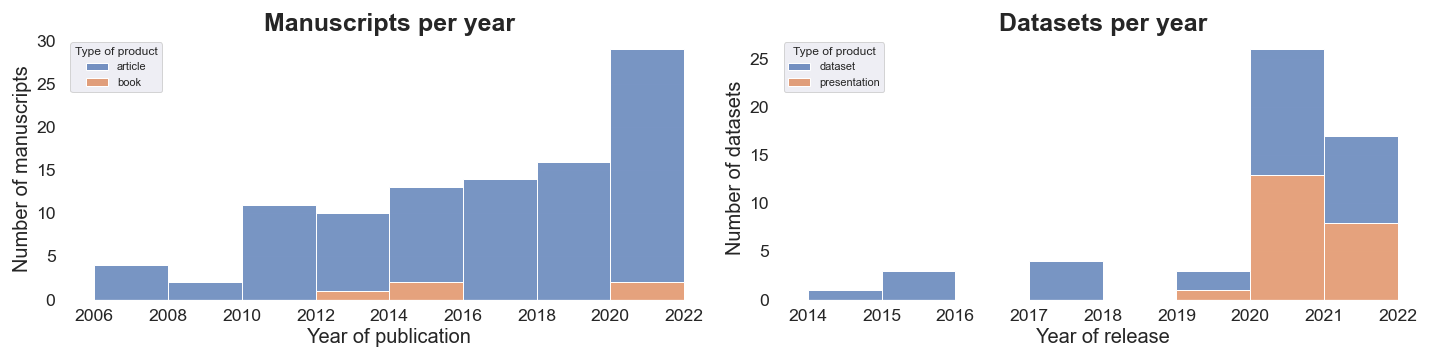
\includegraphics[width=\textwidth]{img/products_per_year.png}
\end{figure}

{\normalfont Nella maggior parte delle mie pubblicazioni in riviste internazionali peer-reviewed, sono elencato come \textbf{primo o ultimo} (senior) autore, a indicare il mio ruolo principale nella ricerca e nella mentorship relativi a questi progetti. Il mio nome appare in posizione prominente nelle liste degli autori, sottolineando il mio significativo contributo alle pubblicazioni di cui sono co-autore. Molti dei miei lavori presentano \textbf{studenti o ricercatori post-dottorato come autori}, evidenziando il mio impegno nello sviluppo della prossima generazione di scienziati.}

\begin{figure}[h]
\centering
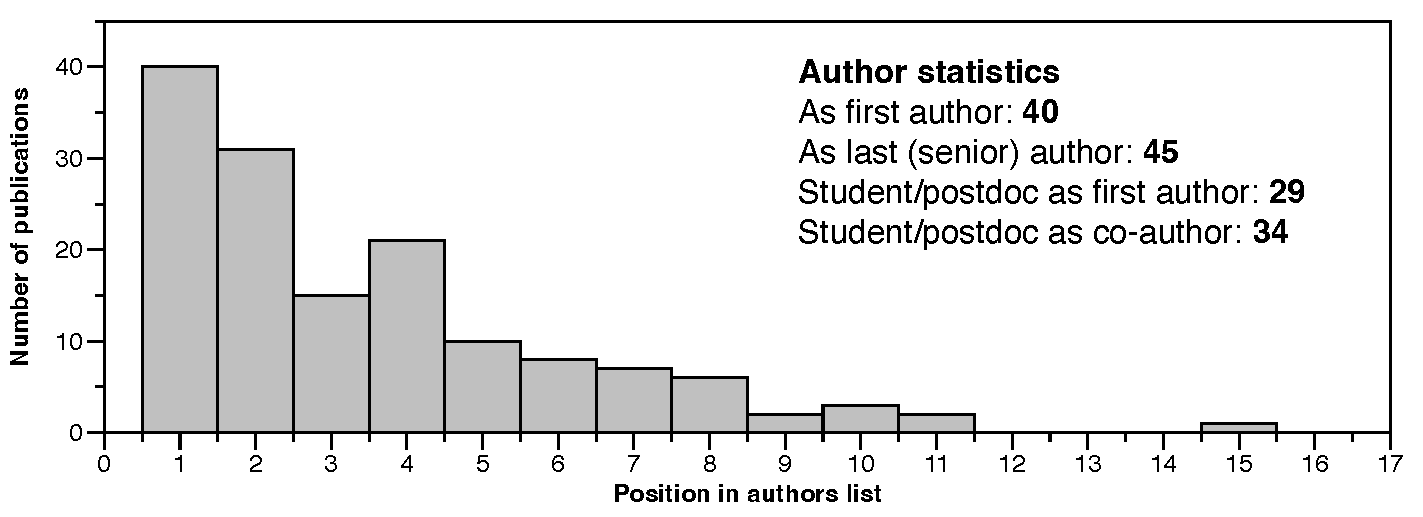
\includegraphics[width=\textwidth]{img/Manuscripts.pdf}
\end{figure}

{\normalfont Ho \textbf{107 documenti} elencati su Scopus, con \textbf{4,253 citazioni} e un \textbf{h-index di 38}. Questi indicatori sono leggermente superiori su Google Scholar, in quanto questa piattaforma considera un'ampia gamma di prodotti di ricerca. Su Web of Science, i miei dati sono distribuiti su diversi profili generati automaticamente, il che può influenzare l'accuratezza del conteggio delle citazioni e di altri indicatori.}

\begin{figure}[h]
\centering
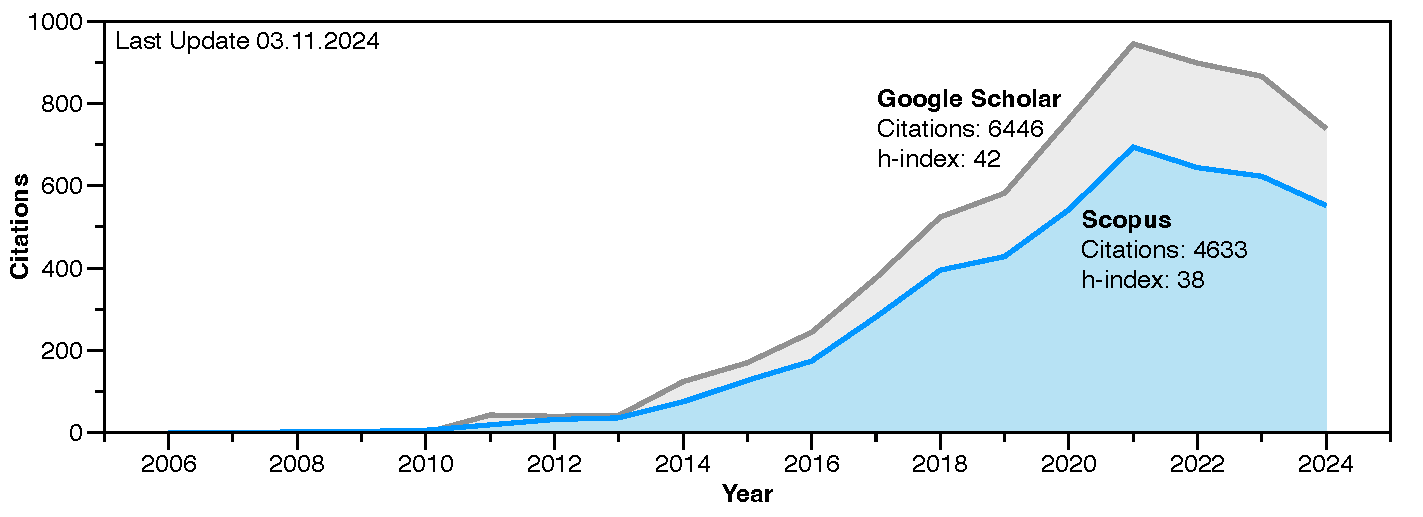
\includegraphics[width=\textwidth]{img/CITATIONS.pdf}
\end{figure}

\newpage

{\normalfont La maggior parte degli articoli di cui sono autore sono stati pubblicati su riviste \textbf{classificate come Q1} dal Journal Citation Reports 2022 (Web of Science), indicando il loro alto impatto e prestigio all'interno della comunità accademica. Il mio output scientifico copre una varietà di riviste, che vanno da pubblicazioni specifiche del settore con impact factor tra 1 e 5, fino a riviste ad alto impatto, con impact factor superiori a 10, secondo il Journal Citation Reports 2022.}

\begin{figure}[h]
\centering
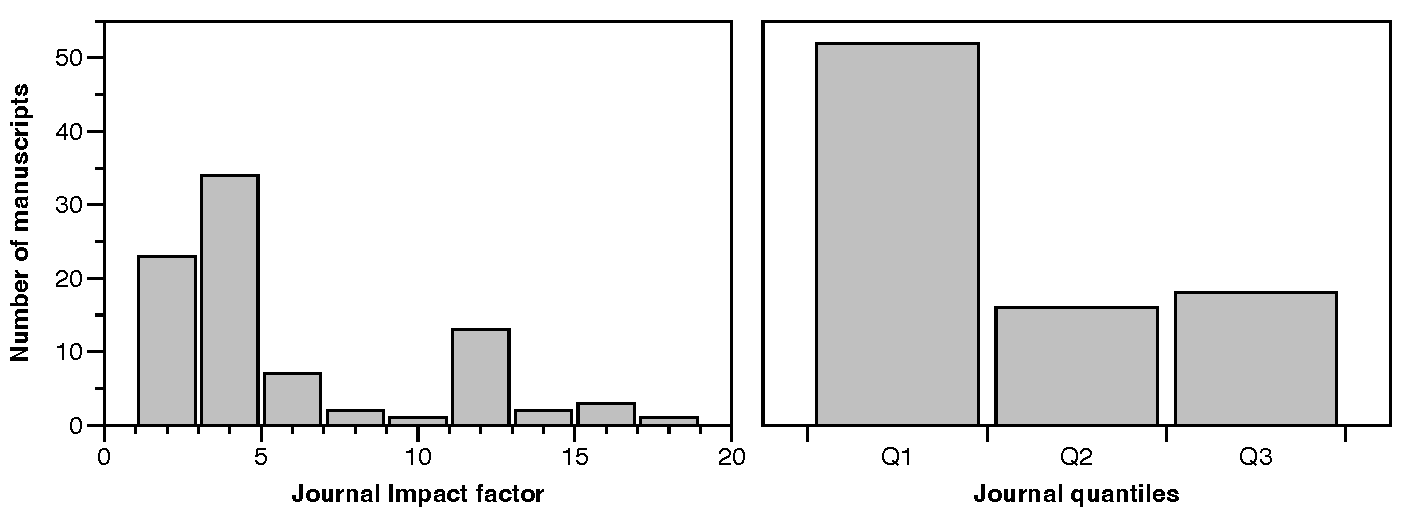
\includegraphics[width=\textwidth]{img/Quantiles.pdf}
\end{figure}

{\normalfont Le riviste in cui pubblico si collocano principalmente nelle categorie di \textbf{geografia fisica e geoscienze}. Inoltre, ho pubblicato in campi strettamente correlati come l'ecologia e la biologia, o il telerilevamento, dimostrando un ampio coinvolgimento in aree di ricerca interdisciplinari.}

\begin{figure}[h]
\centering
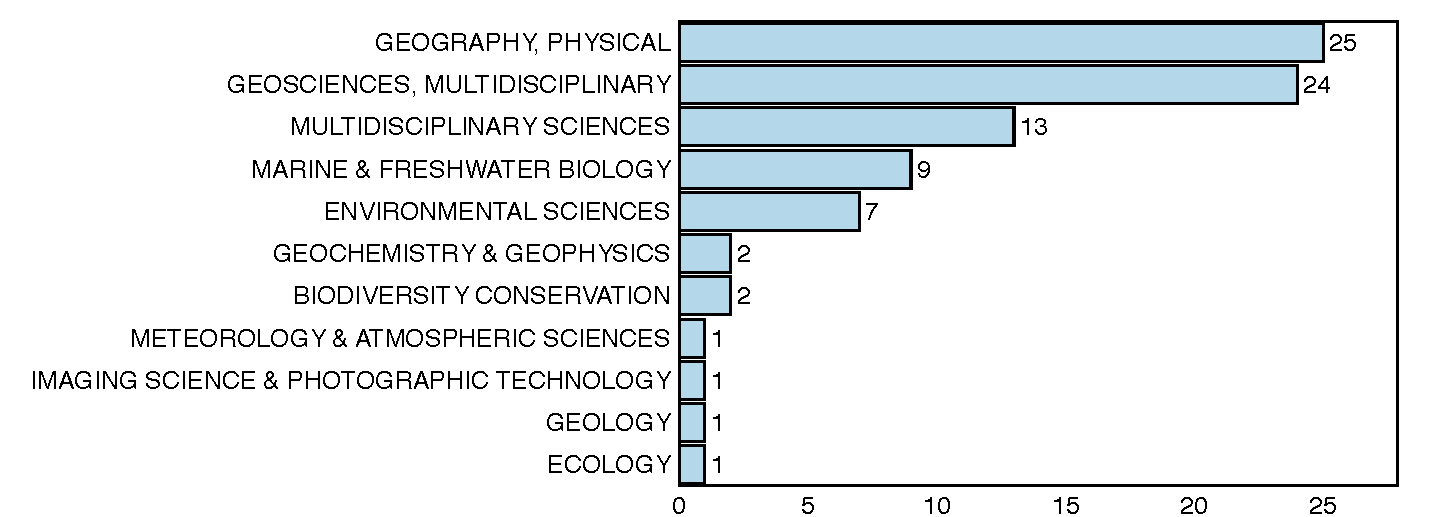
\includegraphics[width=\textwidth]{img/topics.pdf}
\end{figure}
\newpage
{\normalfont Una panoramica dell'impatto delle mie attività di ricerca dal 2013 al 2022 è disponibile su SciVal, una piattaforma sviluppata da Elsevier per l'analisi dei risultati bibliometrici della ricerca. Secondo SciVal, la mia ricerca in questo periodo comprende 74 contributi, che hanno accumulato un totale di 3,493 citazioni. Di seguito sono riportate alcune \textbf{statistiche chiave estratte da SciVal per gli anni 2013 al 2022.}}
\smallskip

{\footnotesize 
\begin{description}
  \item [39.2\%] delle mie pubblicazioni si trovano tra il 10\% più citato a livello mondiale.
  \item [66.7\%] delle mie pubblicazioni sono classificate nel top 10\% delle riviste per CiteScore.
  \item [Q1] 88.4\% delle mie pubblicazioni sono in riviste classificate Q1 da CiteScore, con il resto in riviste Q2.
  \item [2.70] è il mio Field-Weighted Citation Impact (FWCI). Questo indicatore mostra che le mie pubblicazioni ricevono il 170\% di citazioni in più rispetto alla media globale per lavori simili.
\end{description}}

\section{Aree di ricerca}
{\normalfont La mia ricerca copre una vasta gamma di aree geografiche, con un focus sui cambiamenti costieri e del livello del mare. Indago le dinamiche costiere moderne in Germania e Ghana. In località tropicali come Moorea, Tahiti e Fiji, i miei studi esplorano le interazioni tra i processi costieri moderni e le dinamiche ecologiche delle barriere coralline. Inoltre, esamino le variazioni del livello del mare paleo (dal Olocene al Pliocene) in diverse località come il Mediterraneo, Capo Verde, le Bahamas, Aruba, Curaçao, Bonaire, Madagascar, Bermuda, Argentina, Brasile, Seychelles, Sud Africa e Indonesia. Il mio lavoro include anche lo studio della topografia sottomarina delle barriere coralline nelle Maldive e i cambiamenti del livello del mare passati sulla costa est degli Stati Uniti durante il Pliocene e il Pleistocene. Utilizzo una varietà di metodologie per affrontare le complessità legate allo studio della geomorfologia marina e costiera in questi siti distribuiti a livello globale. Ho guidato spedizioni di ricerca in tutte le località sopra menzionate, supervisionando la logistica, ottenendo i permessi di ricerca e organizzando scientificamente il lavoro di campo in diverse occasioni.}

\begin{figure}[h]
\centering
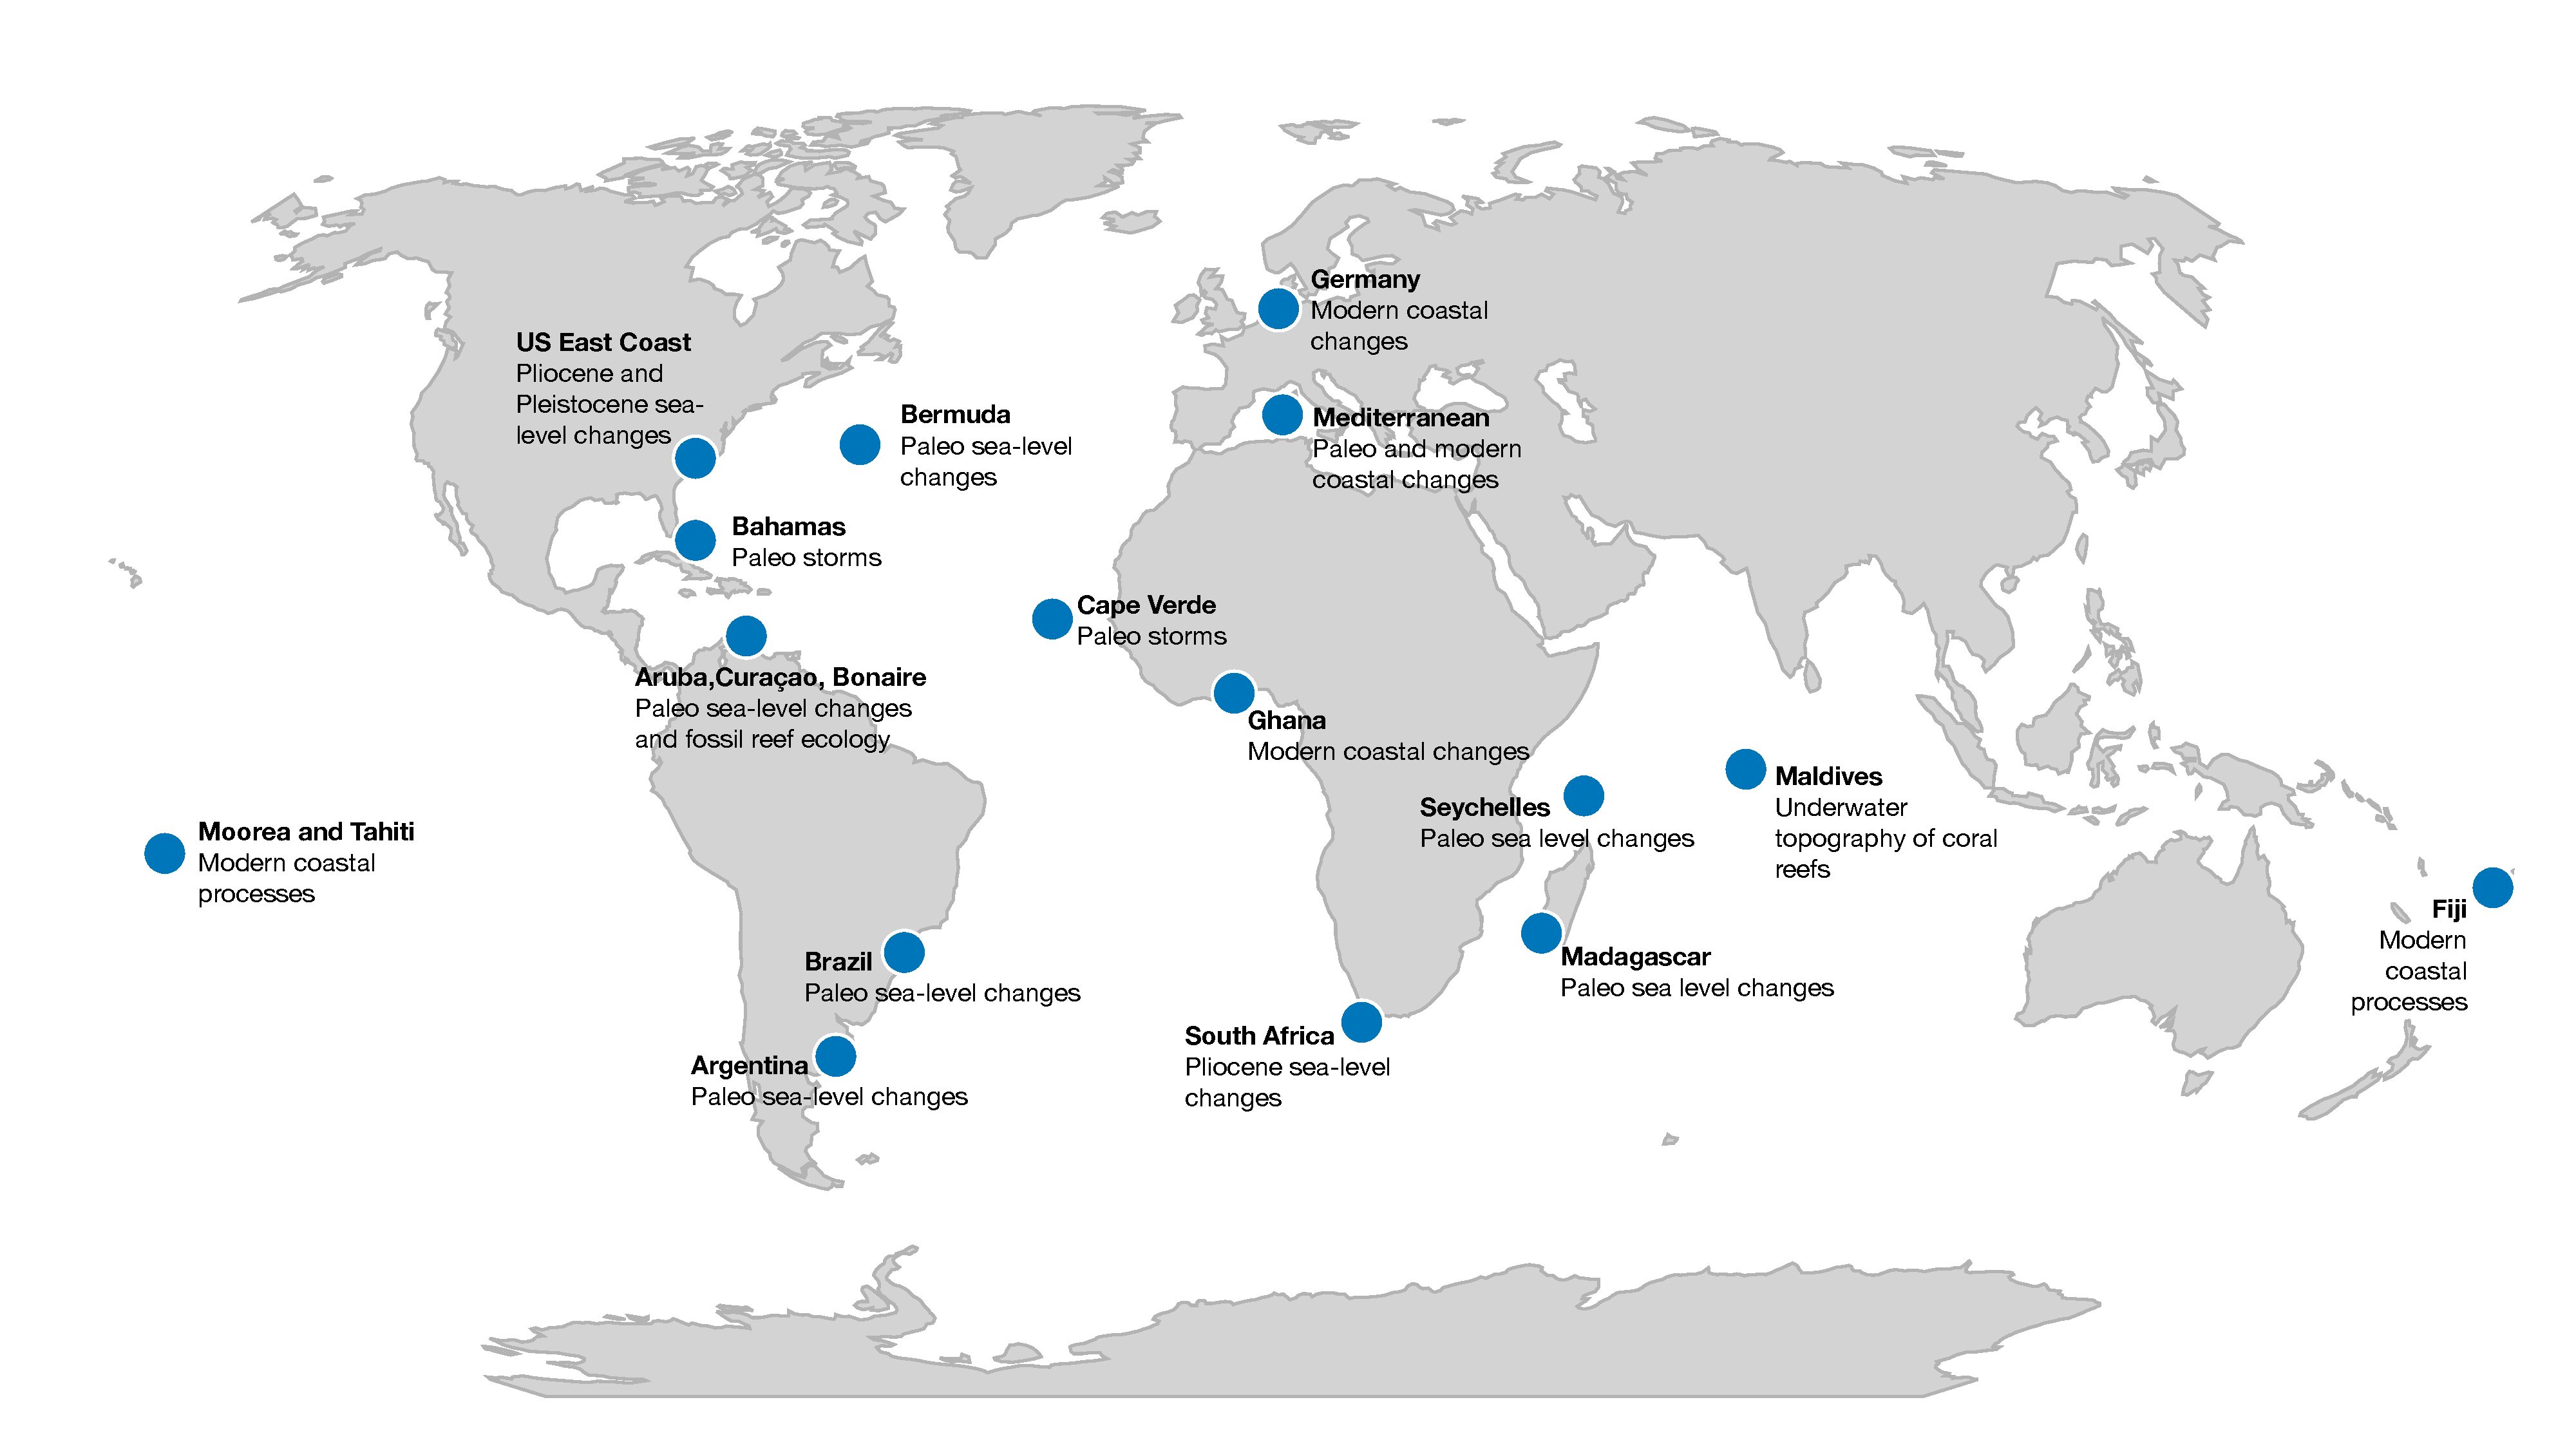
\includegraphics[width=\textwidth]{Research_map/field_data.pdf}
\end{figure}

\newpage
\section{Terza Missione - Rassegna stampa}
{\normalfont Le mie attività di ricerca hanno ricevuto attenzione da parte di vari mezzi di comunicazione, inclusi giornali, stazioni radio, canali televisivi e siti web. Di seguito, fornisco un riepilogo dei principali servizi giornalistici che hanno trattato il mio lavoro.}\\
{\footnotesize 
\begin{description}
  \item [2023] "Ancient warning of a rising sea" (Washington Post, Press, International)
  \item [2023] "Il livello del mare sta salendo. E le nostre coste sono a rischio" (Domani, Press, National) 
  \item [2023] "Ambiente, lo studio: "Livello mare nel 2100 fino a un metro in più rispetto a oggi" (Sky Tg 24, Web Press, National) 
   \item [2023] "Cambiamento climatico e gas serra, nel 2100 il livello del mare può aumentare di un metro: laguna di Venezia sorvegliata speciale" (Il Gazzettino, Web Press, National) 
  \item [2023] "Il nuovo report sul cambiamento climatico: Il mare invaderà certamente le coste, ma possiamo agire per rallentare il fenomeno" (La Stampa, Press, National) 
  \item [2023] "Aruba’s Bocas: home to the rarest fossil reefs on the planet!" (Aruba today, Web Press, International) 
  \item [2022] "Se sparisse il ghiaccio dei Poli..." (Focus, Press, National) 
  \item [2021] "Surprisingly fast ice-melts in past raise fears about sea level rise" (Horizon Magazine, Web Press, National) 
  \item [2021] "E se il mare del passato fosse stato più basso di quanto crediamo?" (Oggiscienza, Press, National) 
  \item [2020] "La sfida delle inondazioni, sempre più violente e frequenti" (Le Scienze, Press, National) 
  \item [2020] "South African seas up to 30m higher show a wet planet under siege" (Daily Maverick, Press, International) 
  \item [2020] "Sea-level rise projections can improve with state-of-the-art model" (Science Daily, Press, International) 
  \item [2017] "Ancient storms could have hurled huge boulders, scientists say" (Washington post, Press, International) 
  \item [2017] "Drohnen liefern detailreiche Einblicke in Korallenriffe" (Der Standard, Press, International) 
  \item [2017] "Mit Drohnen über dem Korallenriff" (Deutschland Radio, Radio, International) 
  \item [2017] "Riffe schützen Inseln vor Monsterwellen. Die Welle" (Die Welle, Web press, International) 
  \item [2017] "Drohnen für die Wissenschaft" (Arte TV, Television, International) 
  \item [2017] "Mit Drohnen gegen die Korallenbleiche" (Welt, Television, International) 
  \item [2016] "I droni contro l’erosione delle coste" (Dronezine, Press, National) 
  \item [2015] "Quatre chercheurs au milieu des surfeurs" (La Depeche de Tahiti, Press, International) 
  \item [2013] "Il business che spinge la startup é l’ecosistema costiero" (Il Secolo XIX, Press, National) 
  \item [2013] "How High Could the Tide Go?" (New York Times, Press, International) 
  \item [2011] "I protagonisti della ricerca scientifica in mare si raccontano" (SubAqua magazine, Press, National) 
\end{description}}

\section{Terza Missione - Divulgazione}
{\normalfont Sono attivamente impegnato nella diffusione del mio lavoro scientifico attraverso la creazione di contenuti sui canali di social media, con un particolare interesse per la comunicazione scientifica. Ad esempio, un recente video che illustra la mia competenza prodotto da Ca' Foscari ha ottenuto circa 67.000 visualizzazioni su TikTok e 29.000 su Instagram.}\\

\bigskip

\subsection{YouTube $|$ {\normalfont\textit{@CoastalScience}}}
{\footnotesize Creo e condivido video che trattano tecniche di campo, sistemi informativi geografici e routine quotidiane di lavoro sul campo. Il mio canale attualmente conta 395 iscritti, e i miei video hanno raggiunto circa 52.000 visualizzazioni, con un tempo di visione totale di quasi 3.000 ore.}
\bigskip

\subsection{Podcast $|$ {\normalfont\textit{Storie di Mare}}}
{\footnotesize Produco e conduco un podcast intitolato "Storie di Mare", che utilizza il racconto per educare gli ascoltatori sui processi costieri e marini. Le mie puntate sono state ascoltate in streaming circa 2.400 volte e sono disponibili su piattaforme come Spotify, YouTube e Amazon Music.}
\bigskip

\subsection{Educazione Ambientale $|$ {\normalfont\textit{Sons of the Ocean}}}
{\footnotesize Collaboro con "Sons of the Ocean", un'organizzazione no-profit dedicata all'educazione ambientale per bambini e giovani in età scolare. Contribuisco con contenuti multimediali, inclusi commenti video per i social media, e tengo presentazioni volte alla divulgazione scientifica.}

\newpage



\begin{center}
    {\fontsize{36}{36}\selectfont\interthin Lista delle \interheavy Pubblicazioni} \\
\bigskip
        {\color{icnclr}} \textit{{I nomi di assegnist*, student* di dottorato e student* magistrali \\ che erano sotto la mia supervisione al momento della pubblicazione sono \underline{sottolineati}.}}

\end{center}

\nocite{*}
\section{Libri e capitoli di libro}
\printbibliography[type=book,heading=none]

\section{Articoli su riviste scientifiche internazionali}
\printbibliography[type=article,heading=none]

\section{Altri articoli peer reviewed}
\printbibliography[type=periodical,heading=none]

\section{Presentazioni selezionate}
\printbibliography[type=dataset,heading=none]
\printbibliography[type=misc,heading=none]


\end{document}